\chapter{Results}

\section{Size exclusion chromatography}

The results of the size exclusion chromatography are shown in figure
\ref{fig:sec} for all three proteins. For each protein, the fractions below the
main peak were pooled for further processing, while the rest was discarded.

\begin{figure}
    \centering
    \begin{subfigure}{0.45\textwidth}
        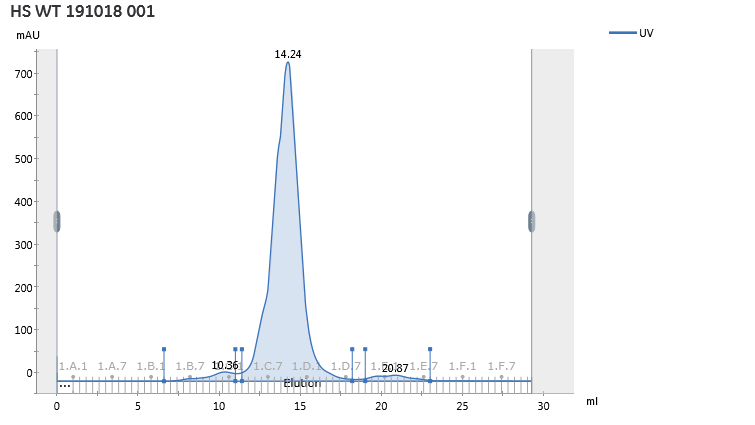
\includegraphics[width=\textwidth]{img/sec_wt}
        \caption{SEC graph of wildtype}
        \label{fig:sec_wt}
    \end{subfigure}
    ~
    \begin{subfigure}{0.45\textwidth}
        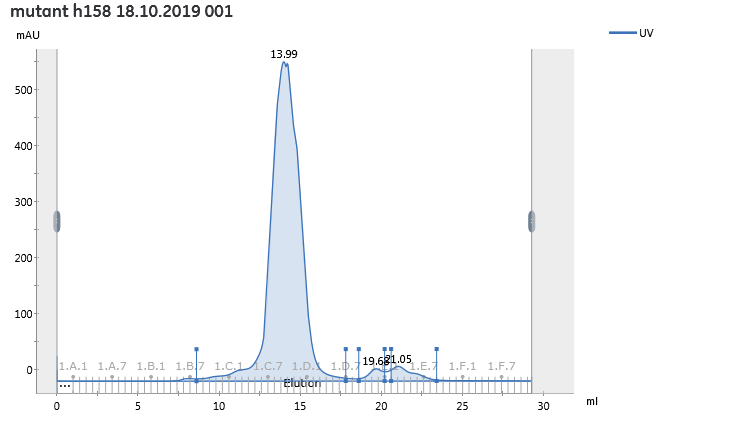
\includegraphics[width=\textwidth]{img/sec_mut}
        \caption{SEC graph of mutant}
        \label{fig:sec_mut}
    \end{subfigure}

    \begin{subfigure}{0.45\textwidth}
        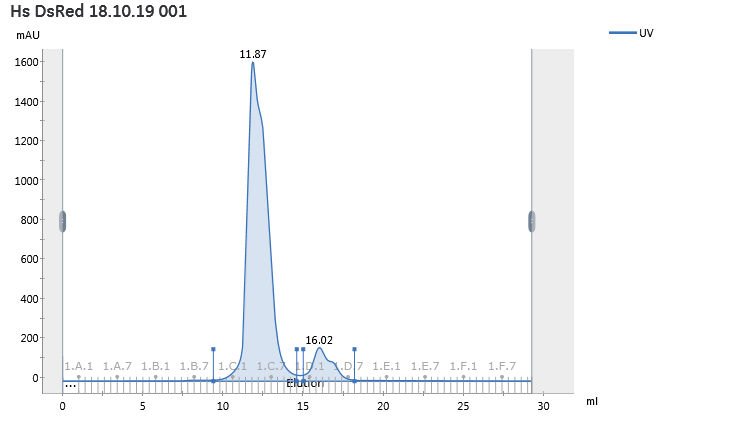
\includegraphics[width=\textwidth]{img/sec_dsred}
        \caption{SEC graph of dsRed}
        \label{fig:sec_dsred}
    \end{subfigure}
    \caption{SEC graphs of three SOO variants}
    \label{fig:sec}
\end{figure}

\section{Protein concentration determination}

Figure \ref{fig:hs_concentration} shows the absorption of the three protein
samples at various wavelengths. The absorption of use to us is the one at
\SI{561}{\nm} which is the absorbance of the two hemes within SOO.

In a first step, the absorption difference at \SI{561}{\nm} between the
oxidated and reduced forms was calculated. In order to compensate the fact that
the baseline of the reduced form was lower, the average absorption difference
in the range of \SIrange{580}{600}{\nm} was calculated, and added to the
previously calculated absorption difference at \SI{561}{\nm}.

Finally, using the path length of the cuvette of \SI{1}{\cm}, the provided
extinction coefficient of \SI{46.36}{\per\milli\Molar\per\cm} and the dilution
factor of \SI{375} the protein concentration was calculated using Beer's law.
These metrics including the final concentration are shown in table
\ref{tbl:hs_concentration}.

\begin{figure}
	\centering
	\includegraphics[width=0.9\textwidth]{img/hs_concentration.png}
	\caption{Absorption of HS for concentratoin determination}
	\label{fig:hs_concentration}
\end{figure}

\begin{table}
	\centering
	\begin{tabu}{lllll}
		\toprule
		Protein & $\Delta_{\text{Absorption at \SI{561}{\nm}}}$ & Baseline & $\Delta_{\text{Absorption at \SI{561}{\nm} corr}}$ & Concentration [\si{\milli\Molar}] \\
		\midrule
		Wildtype & 0.042 & 0.004 & 0.046 & 0.372 \\
		Mutant & 0.043 & 0.006 & 0.049 & 0.396 \\
		dsRed & 0.068 & 0.013 & 0.081 & 0.655 \\
		\bottomrule
	\end{tabu}
	\caption{Concentration of purified HS}
	\label{tbl:hs_concentration}
\end{table}

\section{SDS PAGE}

The results of the SDS page gels are shown in figure \ref{fig:sds}.

\begin{figure}
    \centering
    \begin{subfigure}{0.45\textwidth}
        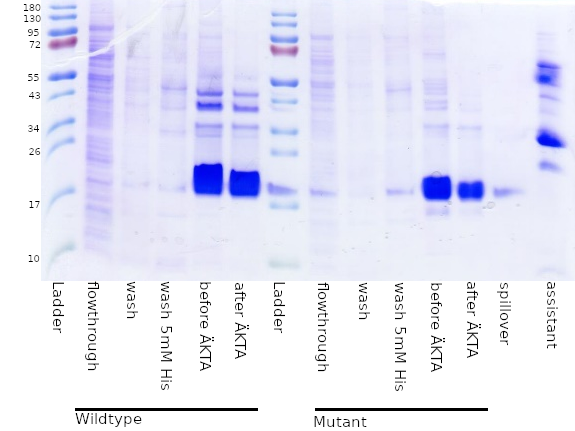
\includegraphics[width=\textwidth]{img/sds_wt_mut}
        \caption{SDS PAGE gel of wildtype and mutant}
        \label{fig:sds_wt_mut}
    \end{subfigure}
    ~
    \begin{subfigure}{0.45\textwidth}
        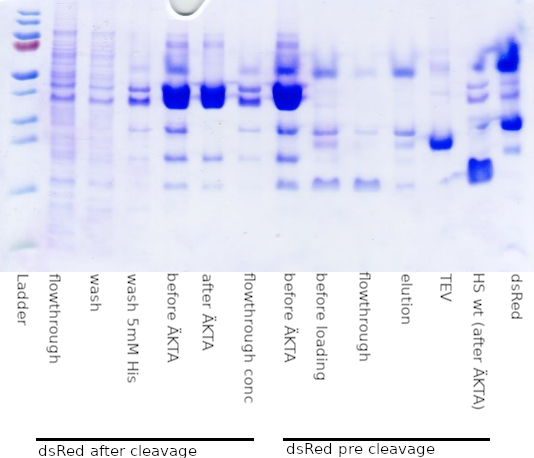
\includegraphics[width=\textwidth]{img/sds_dsred_tev_cleavage.png}
        \caption{SDS PAGE gel of dsRed including cleaved dsRed}
        \label{fig:sds_wt_mut}
    \end{subfigure}
    \caption{SDS gels of three protein variants}
    \label{fig:sds}
\end{figure}

\chapter{Discussion}

\section{Size exclusion chromatography}

In all three SEC graphs there are peaks next to the main one, which imply that
there were impurities within the column. Impurities which are in later
fractions than SOO took longer to pass through the columns, hence contain
molecules which are smaller than SOO. Similarly impurities which are in earlier
fractions are larger than SOO.

This step allowed to further purify the protein, allowing to filter not only on
the affinity to nickel beads as was done before, but in addition to filter
based on the size of molecules.

\section{Protein concentration determination}

The determined concentration of the wild type and mutant is comparable, while
the one of dsRed is significantly bigger. This matches the observation that the
dsRed pellet at the beginning of purification was heavier.

\section{SDS PAGE}

In all three samples the flowthrough contained many compounds of different
size. These were all compounds which were unable to bind to the column, hence
which did not have a His tag.

The wash samples of the wildtype and mutant did not contain a lot, whereas the
one of dsRed contained a variety of compounds found both in the flowthrough, as
well as in later stages. This might imply that the column used for dsRed had
been loaded above capacity.

The \SI{5}{\milli\Molar} His wash allowed to wash out everything which was able
to weakly bind to the column, without washing up the strongly bound SOO.
Comparing the bands with the bands from later purification steps which are
known to be SOO imply that a bit of SOO was washed out in this step.

The before ÄKTA lanes were the result of the elution of the column with
\SI{100}{\milli\Molar} His. The big bands are likely the HS. Of interest is
that, for the wildtype and mutant the big bands are around \SI{17}{\kilo\Da},
while for dsRed they are around \SI{43}{\kilo\Da}. This implies that the dsRed
HS forms trimers. As this behaviour is only seen in small amounts for the
wildtype, and barely for the mutant, dsRed itself seems to promote formation of
these trimers.
